%%% Fiktivní kapitola s ukázkami sazby
\chapter{Analýza existujících řešení}\label{chap:analysis}

Funkcionalita systému, který vyvíjíme, není ve světě software zcela unikátní a~systém, jako samostatný produkt, by ani nebyl příliš hodnotný.
Jak už jsme si ale představili v~úvodní kapitole \ref{chap:intro}, \textit{Firma} si žádá vlastní implementaci systému, kvůli požadavkům na jednoduchost použití a~pozdější propojení s~dalšími produkty \textit{firmy} (o~tom více v~kapitole \nameref{chap:requirements}).

Přesto se pojďme podívat na možnosti řešení tohoto problému v~mírně obecnější rovině, kdy se budeme soustředit jen na vybrané požadavky \textit{Firmy}, abychom dokázali vyvíjený systém zasadit do kontextu již existujícího software.
Budeme se snažit najít již existující softwarový systém či jejich kombinaci, která se v~rámci nabízené funkcionality blíží 3 vybraným funkčním požadavkům, systém tedy umožní:

\begin{enumerate}
    \item grafické mapování dat mezi zákaznickou databází a~generickým datovým modelem, aby bylo možné vytvořit sadu SQL Views transformující zákaznické data na generickým datovým modelem,
    \item vytváření základních reportů, které lze přenášet mezi zákazníky, aby tato činnost nemusela být vykonávána manuálně,
    \item a~běžnou BI funkcionalitu (vizualizaci dat, vytváření reportů, atd.).
\end{enumerate}

Jelikož se nepodařilo najít jeden systém, který by splňoval všechny tři výše uvedené požadavky, budeme muset uvažovat o~kombinaci dvou či více systémů.
První požadavek nejlépe odpovídá kategorii nástrojů pro integraci dat, zbylé dva požadavky odpovídají právě BI nástrojům.
Tyto dvě kategorie si představíme v~následujících dvou sekcích:

\begin{enumerate}
    \item \nameref{sec:DatInteg}
    \item \nameref{sec:BITools}
\end{enumerate}

V sekci \ref{sec:AnalysEnd} si provedenou analýzu možných řešení shrneme.

\section{Integrace dat}\label{sec:DatInteg}

Nástrojů pro integraci dat je mnoho, některá řešení jsou kvalitnější a~jiná méně.
Využijeme-li srovnání nástrojů na integraci dat od porandetské společenosti Gartner\cite{FIG:DatInteg}, které je ilustrované na obrázku \ref{fig:datInteg}, a~aplikujeme podmínku č.~1 z~úvodního textu této kapitoly, můžeme výběr zúžit na nástroje:
\begin{itemize}
    \item MS-SQL Server Integration Services
    \item a Talend Open Studio.
\end{itemize}

\begin{figure}
    \centering
    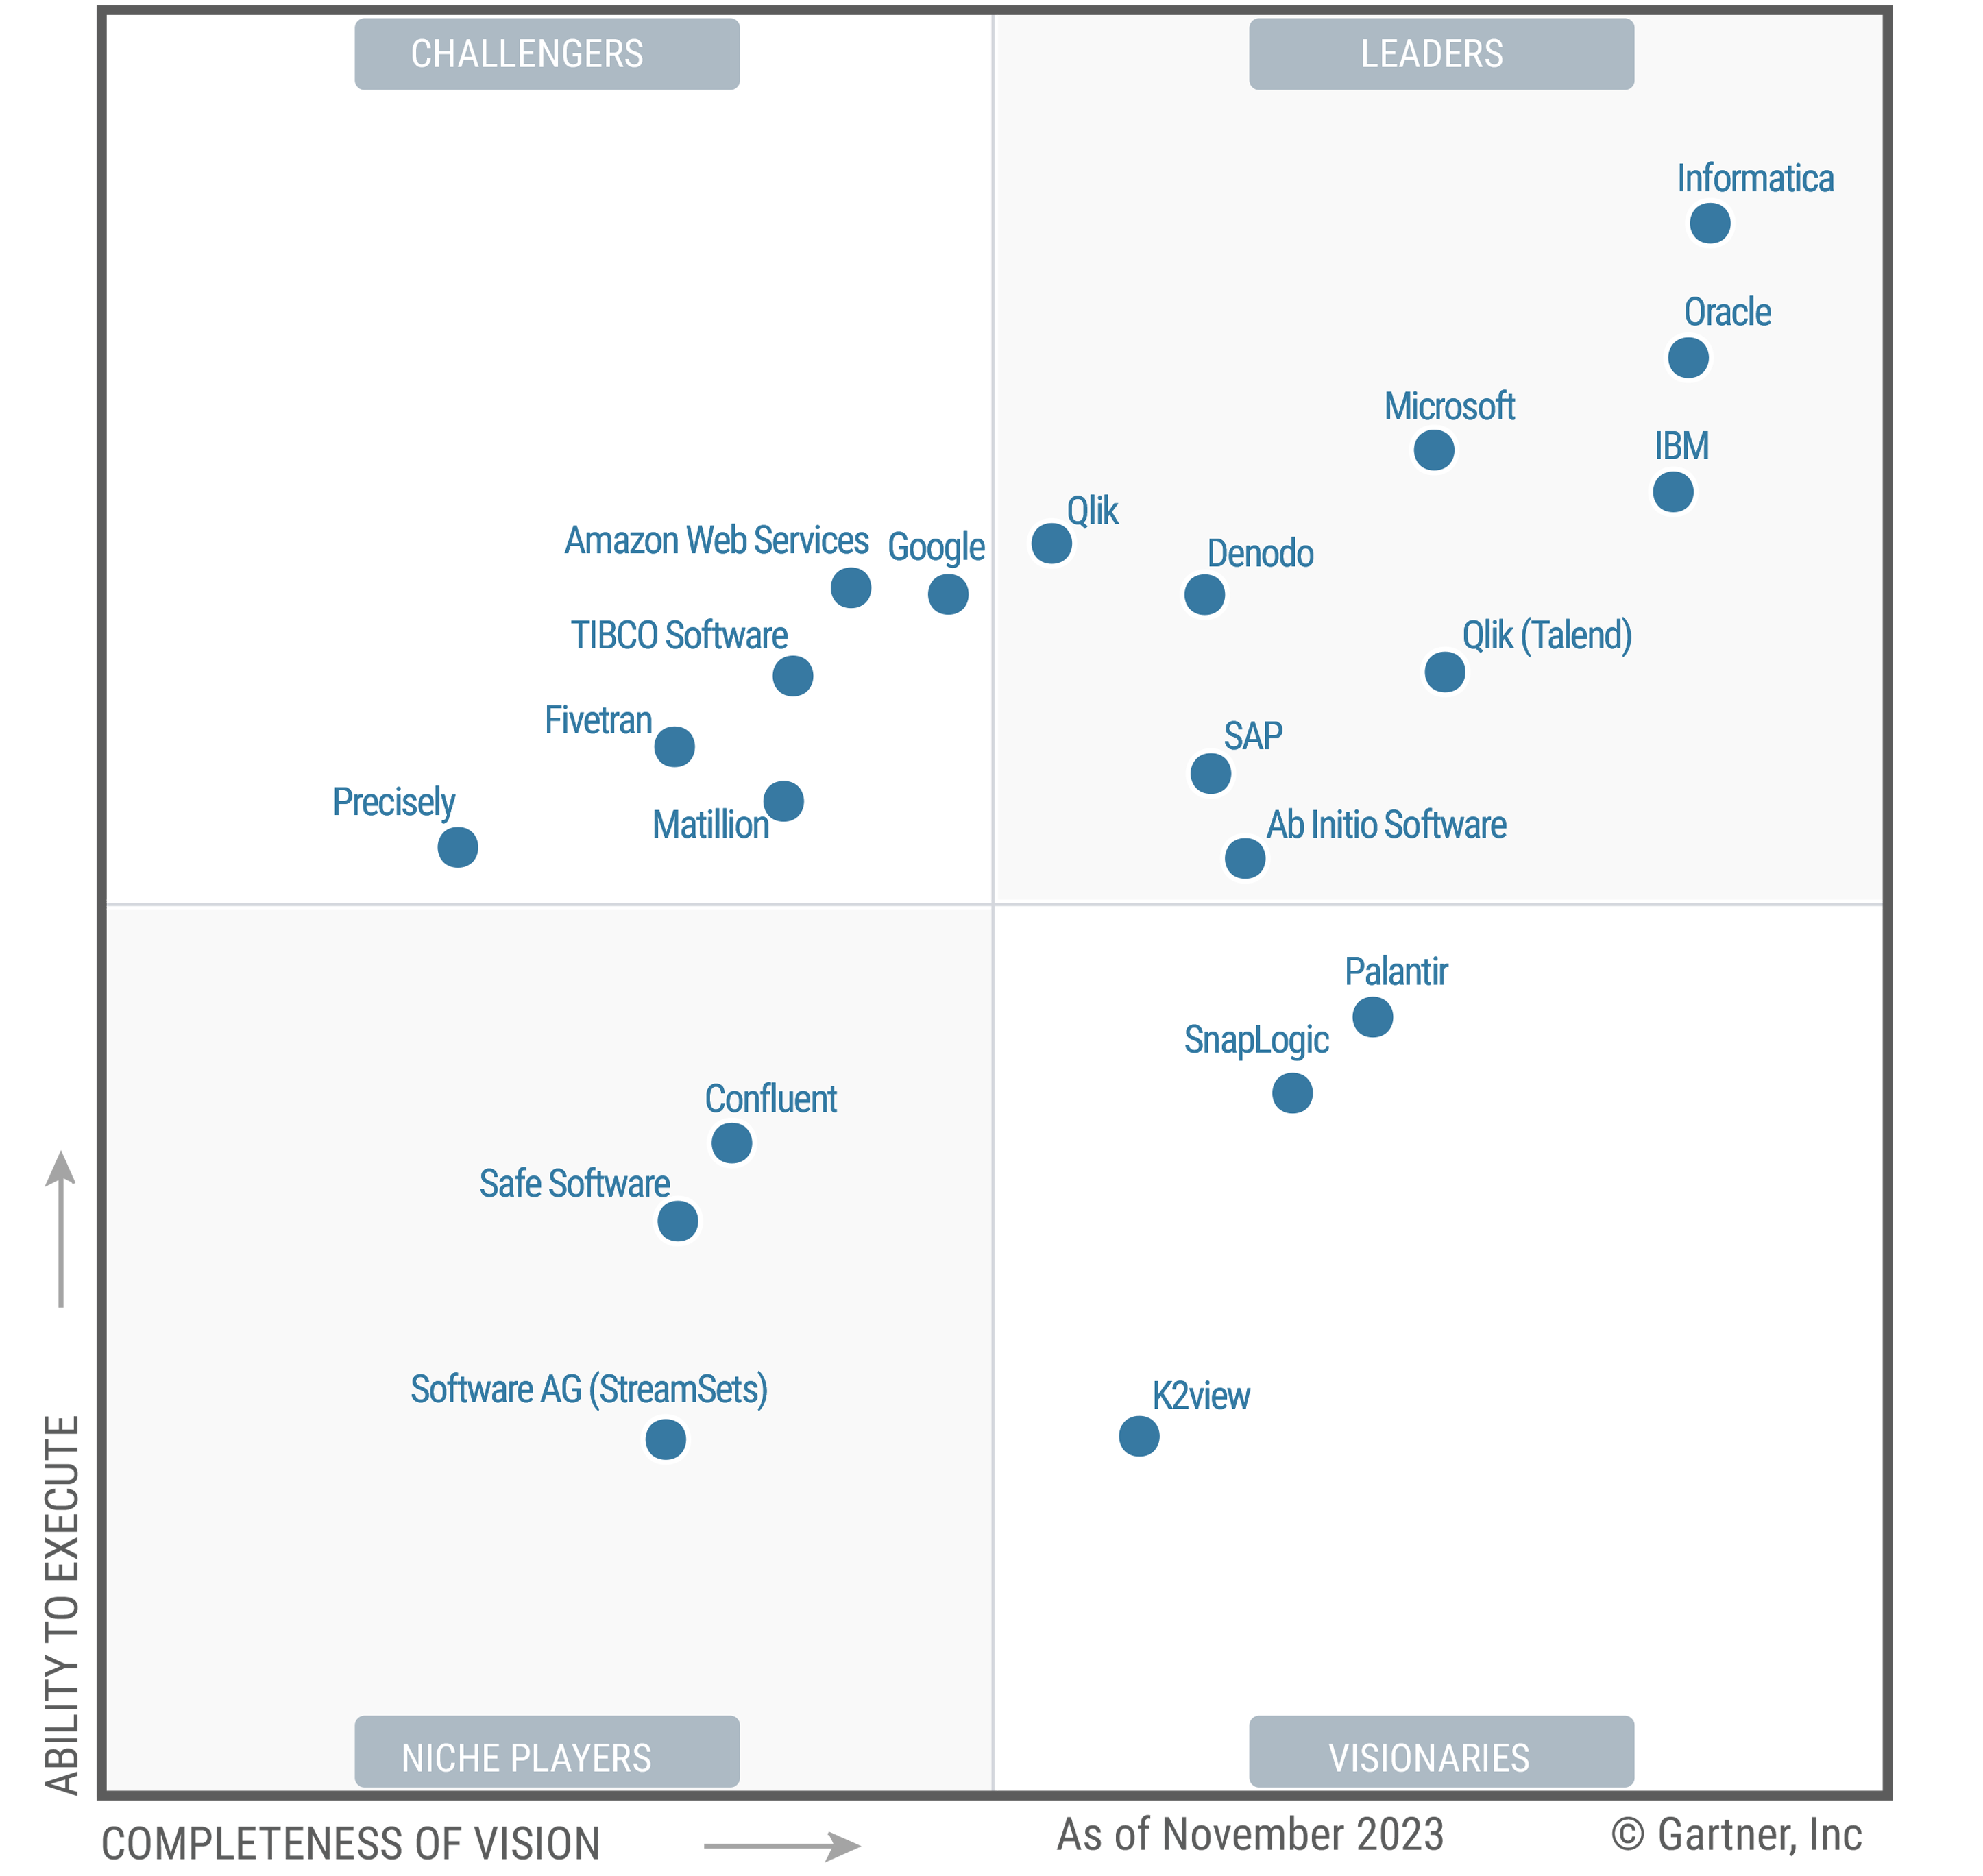
\includegraphics[width=0.75\linewidth]{img/gartner-data-integration.png}
    \caption{Gartner Data integration Magic Quadrant, zdroj: Gartner, 2023}
    \label{fig:datInteg}
\end{figure}

Tyto nástroje si podrobněji rozebereme a vzájemně porovnáme jejich schopnost splnit zmíněnou podmínku č. 1.

\subsection{MS-SQL Server Integration Services (SSIS)}

Microsoft SQL Server Integration Services (SSIS) je platforma pro vývoj podnikových řešení pro extrakci, transformaci a načítání dat (ETL). SSIS je součástí produktu Microsoft SQL Server, což je databázový a~analytický systém\footnote{Více informací na \url{https://www.microsoft.com/en-us/sql-server}}.

\subsubsection{Extrakce dat}
SSIS umožňuje extrakci dat z různých zdrojů, jako jsou relační databáze, XML soubory, webové služby a~další \cite{SQLServerDataSources:online}.
Tento proces je zásadní pro shromažďování dat z~různých zdrojů do jednoho úložiště ve formě, která je vhodná pro další zpracování.

\subsubsection{Transformace dat} Po extrakci dat SSIS poskytuje nástroje pro čištění, normalizaci, agregaci a další transformace dat. To zahrnuje operace jako spojení dat, rozdělení dat, nahrazení hodnot a~mapování dat \cite{SSISDataMapping:online}, pro což SSIS nabízí vizualní editor, jak ilustruje obrázek \ref{fig:SSISColumnMapping}.

\begin{figure}
    \centering
    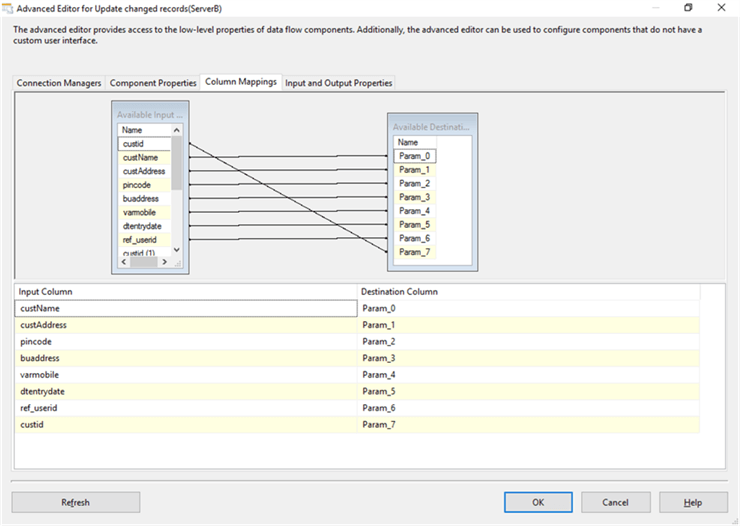
\includegraphics[width=0.75\linewidth]{img/SSIS column mapping.png}
    \caption{Mapování sloupců v SSIS, zdroj: Patel Bhavesh, 2017, dostupné z \url{https://www.mssqltips.com/tipimages2/5082_synchronization-jtk.012.png}}
    \label{fig:SSISColumnMapping}
\end{figure}

\subsubsection{Automatizace a orchestrace} SSIS také poskytuje nástroje pro automatizaci a orchestraci\footnote{Více na \url{https://cs.wikipedia.org/wiki/Orchestrace_(informatika)}} celého procesu ETL. To zahrnuje plánování úloh, sledování výkonu a řízení chyb.

\subsubsection{Integrace s dalšími nástroji Microsoft} Jako součást ekosystému Microsoft SQL Server SSIS se dobře integruje s dalšími nástroji Microsoft, jako jsou SQL Server Analysis Services (SSAS) a~SQL Server Reporting Services (SSRS).

\subsubsection{Vytvoření SQL view}
Pomocí grafického editoru SSIS Designer můžeme přehledně vytvářet integrační balíčky\cite{SSISDesigner:online}, prostředí SSIS Designer ilustruje obrázek \ref{fig:SSISDesigner}.
Tyto balíčky lze dle návodu z~edukačních stránek Microsoftu publikovat jako SQL View \cite{SSISViews:online}. 

Tímto postupem lze splnit 1. první funkční požadavek definovaný v~úvodním textu této kapitoly.

\begin{figure}
    \centering
    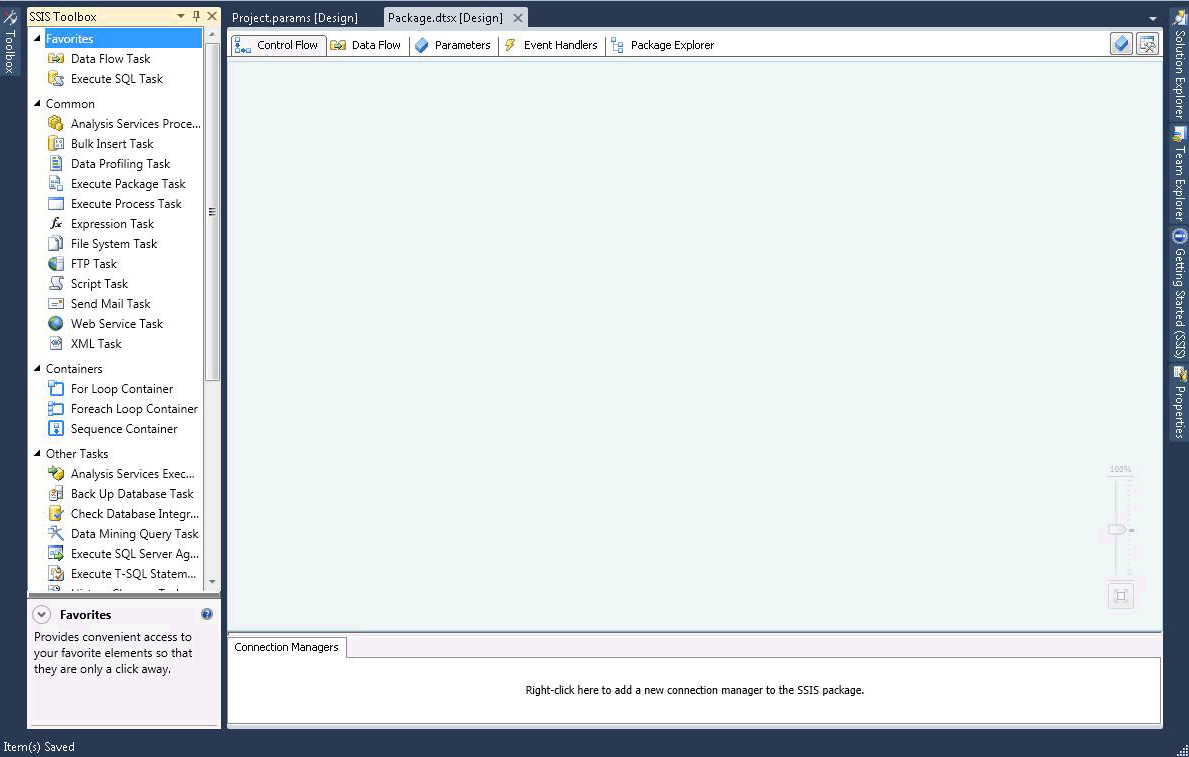
\includegraphics[width=0.75\linewidth]{img/SSIS Designer.png}
    \caption{Prostředí nástroje SSIS Designer, zdroj: Microsoft, 2023, dostupné z: \url{https://learn.microsoft.com/en-us/sql/integration-services/media/denali-designerandtoolbox.gif}}
    \label{fig:SSISDesigner}
\end{figure}

\subsubsection{Shrnutí}
MS-SQL Server Integration Services je silný nástroj pro podnikové ETL řešení a mimo jiné i pro náš případ.
Jeho schopnosti extrakce, transformace a načítání dat, spolu s funkcemi pro automatizaci a integraci s dalšími nástroji Microsoft, z něj činí jeden z klíčových nástrojů pro správu a analýzu dat.


\subsection{Talend Open Studio}

Talend Open Studio je open-source platforma pro vývoj řešení pro extrakci, transformaci a načítání dat (ETL). Tento nástroj je široce používán pro správu dat.

\subsubsection{Extrakce dat}
Talend Open Studio umožňuje extrakci dat z různých zdrojů, jako jsou relační databáze, soubory plochých souborů, webové služby a další. Prostředí nástroje ilustruje obrázek \ref{fig:TalendJobDesigner}

\begin{figure}
    \centering
    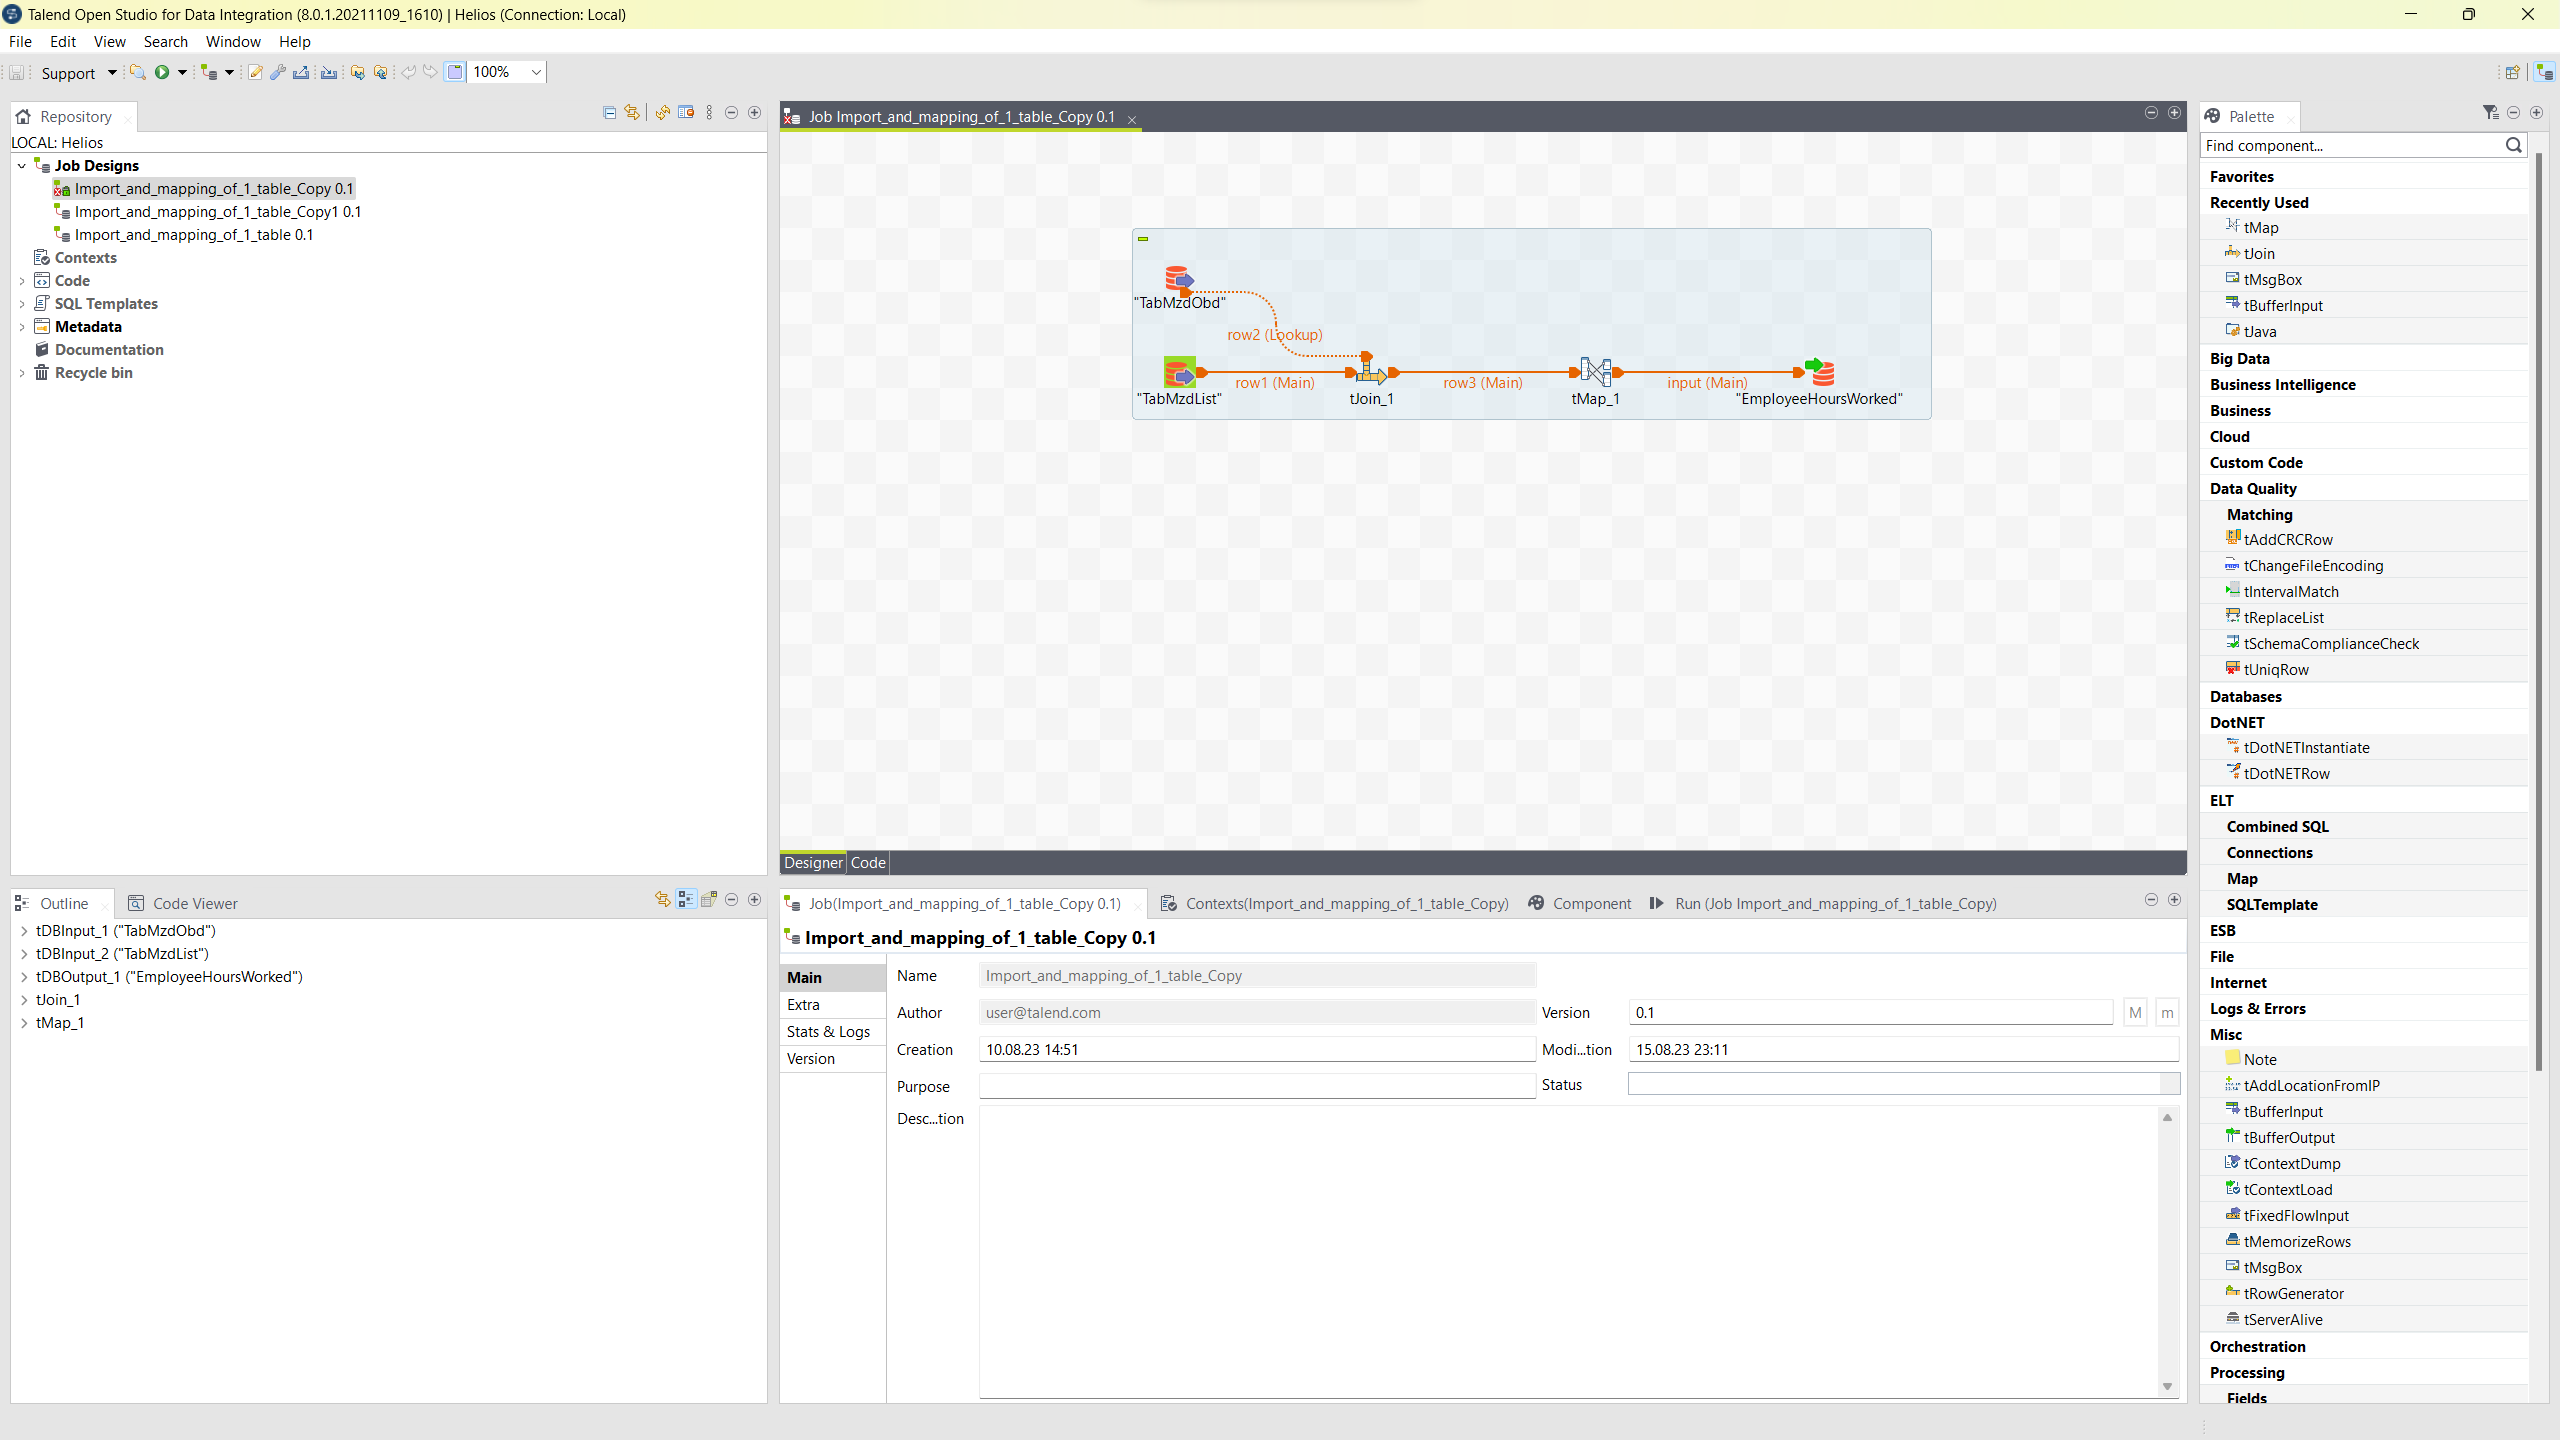
\includegraphics[width=0.75\linewidth]{img/Talend prostředí.png}
    \caption{Prostředí nástroje Talend Open Studio - Job Designer, zdroj: pořízeno autorem práce}
    \label{fig:TalendJobDesigner}
\end{figure}

\subsubsection{Transformace dat}
Po extrakci dat Talend Open Studio poskytuje nástroje pro čištění, normalizaci, agregaci a další transformace dat.
To zahrnuje operace jako spojení dat, rozdělení dat, nahrazení hodnot a také mapování dat, pro což i Open Studio nabízí grafický editor, jak ukazuje obrázek \ref{fig:TalendColumnMapping}.

\begin{figure}
    \centering
    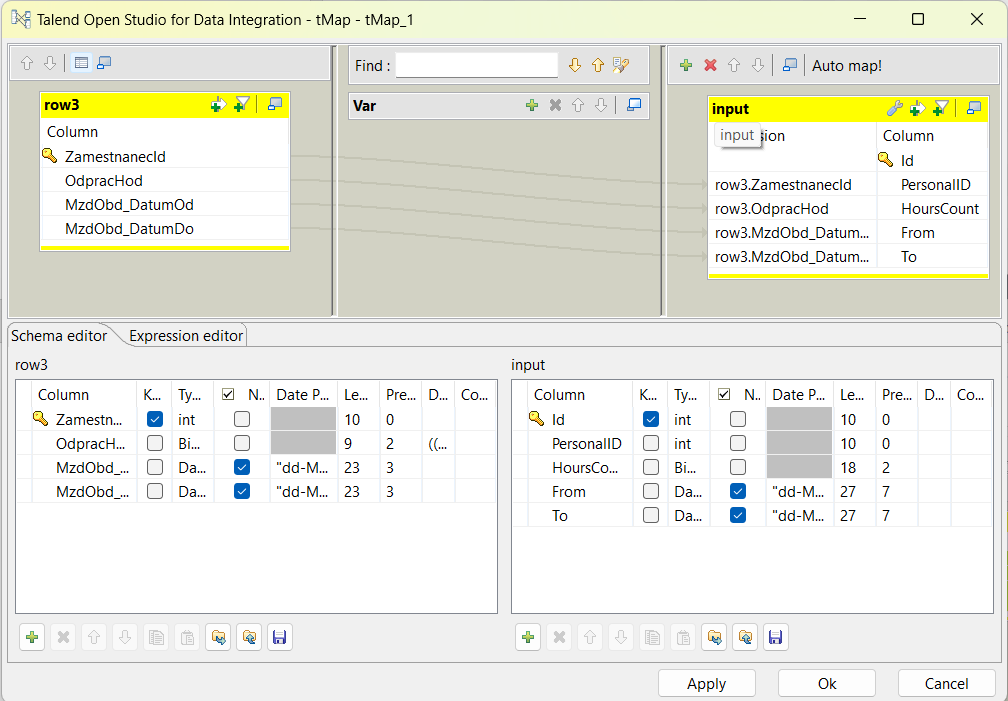
\includegraphics[width=0.6\linewidth]{img/Talend Column mapping.png}
    \caption{Mapování sloupců v Talend Open Studiu, zdroj: pořízeno autorem práce}
    \label{fig:TalendColumnMapping}
\end{figure}

\subsubsection{Automatizace a orchestrace}
Talend Open Studio také poskytuje nástroje pro automatizaci a orchestraci celého ETL procesu. To zahrnuje plánování úloh, sledování výkonu a řízení chyb1.

\subsubsection{Integrace s cloudem}
Talend Open Studio je kompatibilní s cloudovými službami, jako je AWS nebo Azure, což umožňuje snadnou škálovatelnost a pružnost.

\subsubsection{Vytvoření SQL view}


\subsubsection{Shrnutí}
Talend Open Studio je silný nástroj pro podnikové řešení ETL. Jeho schopnosti extrakce, transformace a načítání dat, spolu s funkcemi pro automatizaci a integraci s cloudovými službami, z něj činí klíčový nástroj pro správu a analýzu dat.

zdroje:

https://www.talend.com/products/talend-open-studio/

https://www.talend.com/resources/get-started-talend-open-studio-data-integration/


\section{BI nástroje}\label{sec:BITools}

Budeme-li se řídit výběrem firmy Gartner, Inc\cite{FIG:BiTools} a jejich výběrem lídrů v oblasti BI nástrojů, můžeme použít gartner

\begin{figure}[hp]
    \centering
    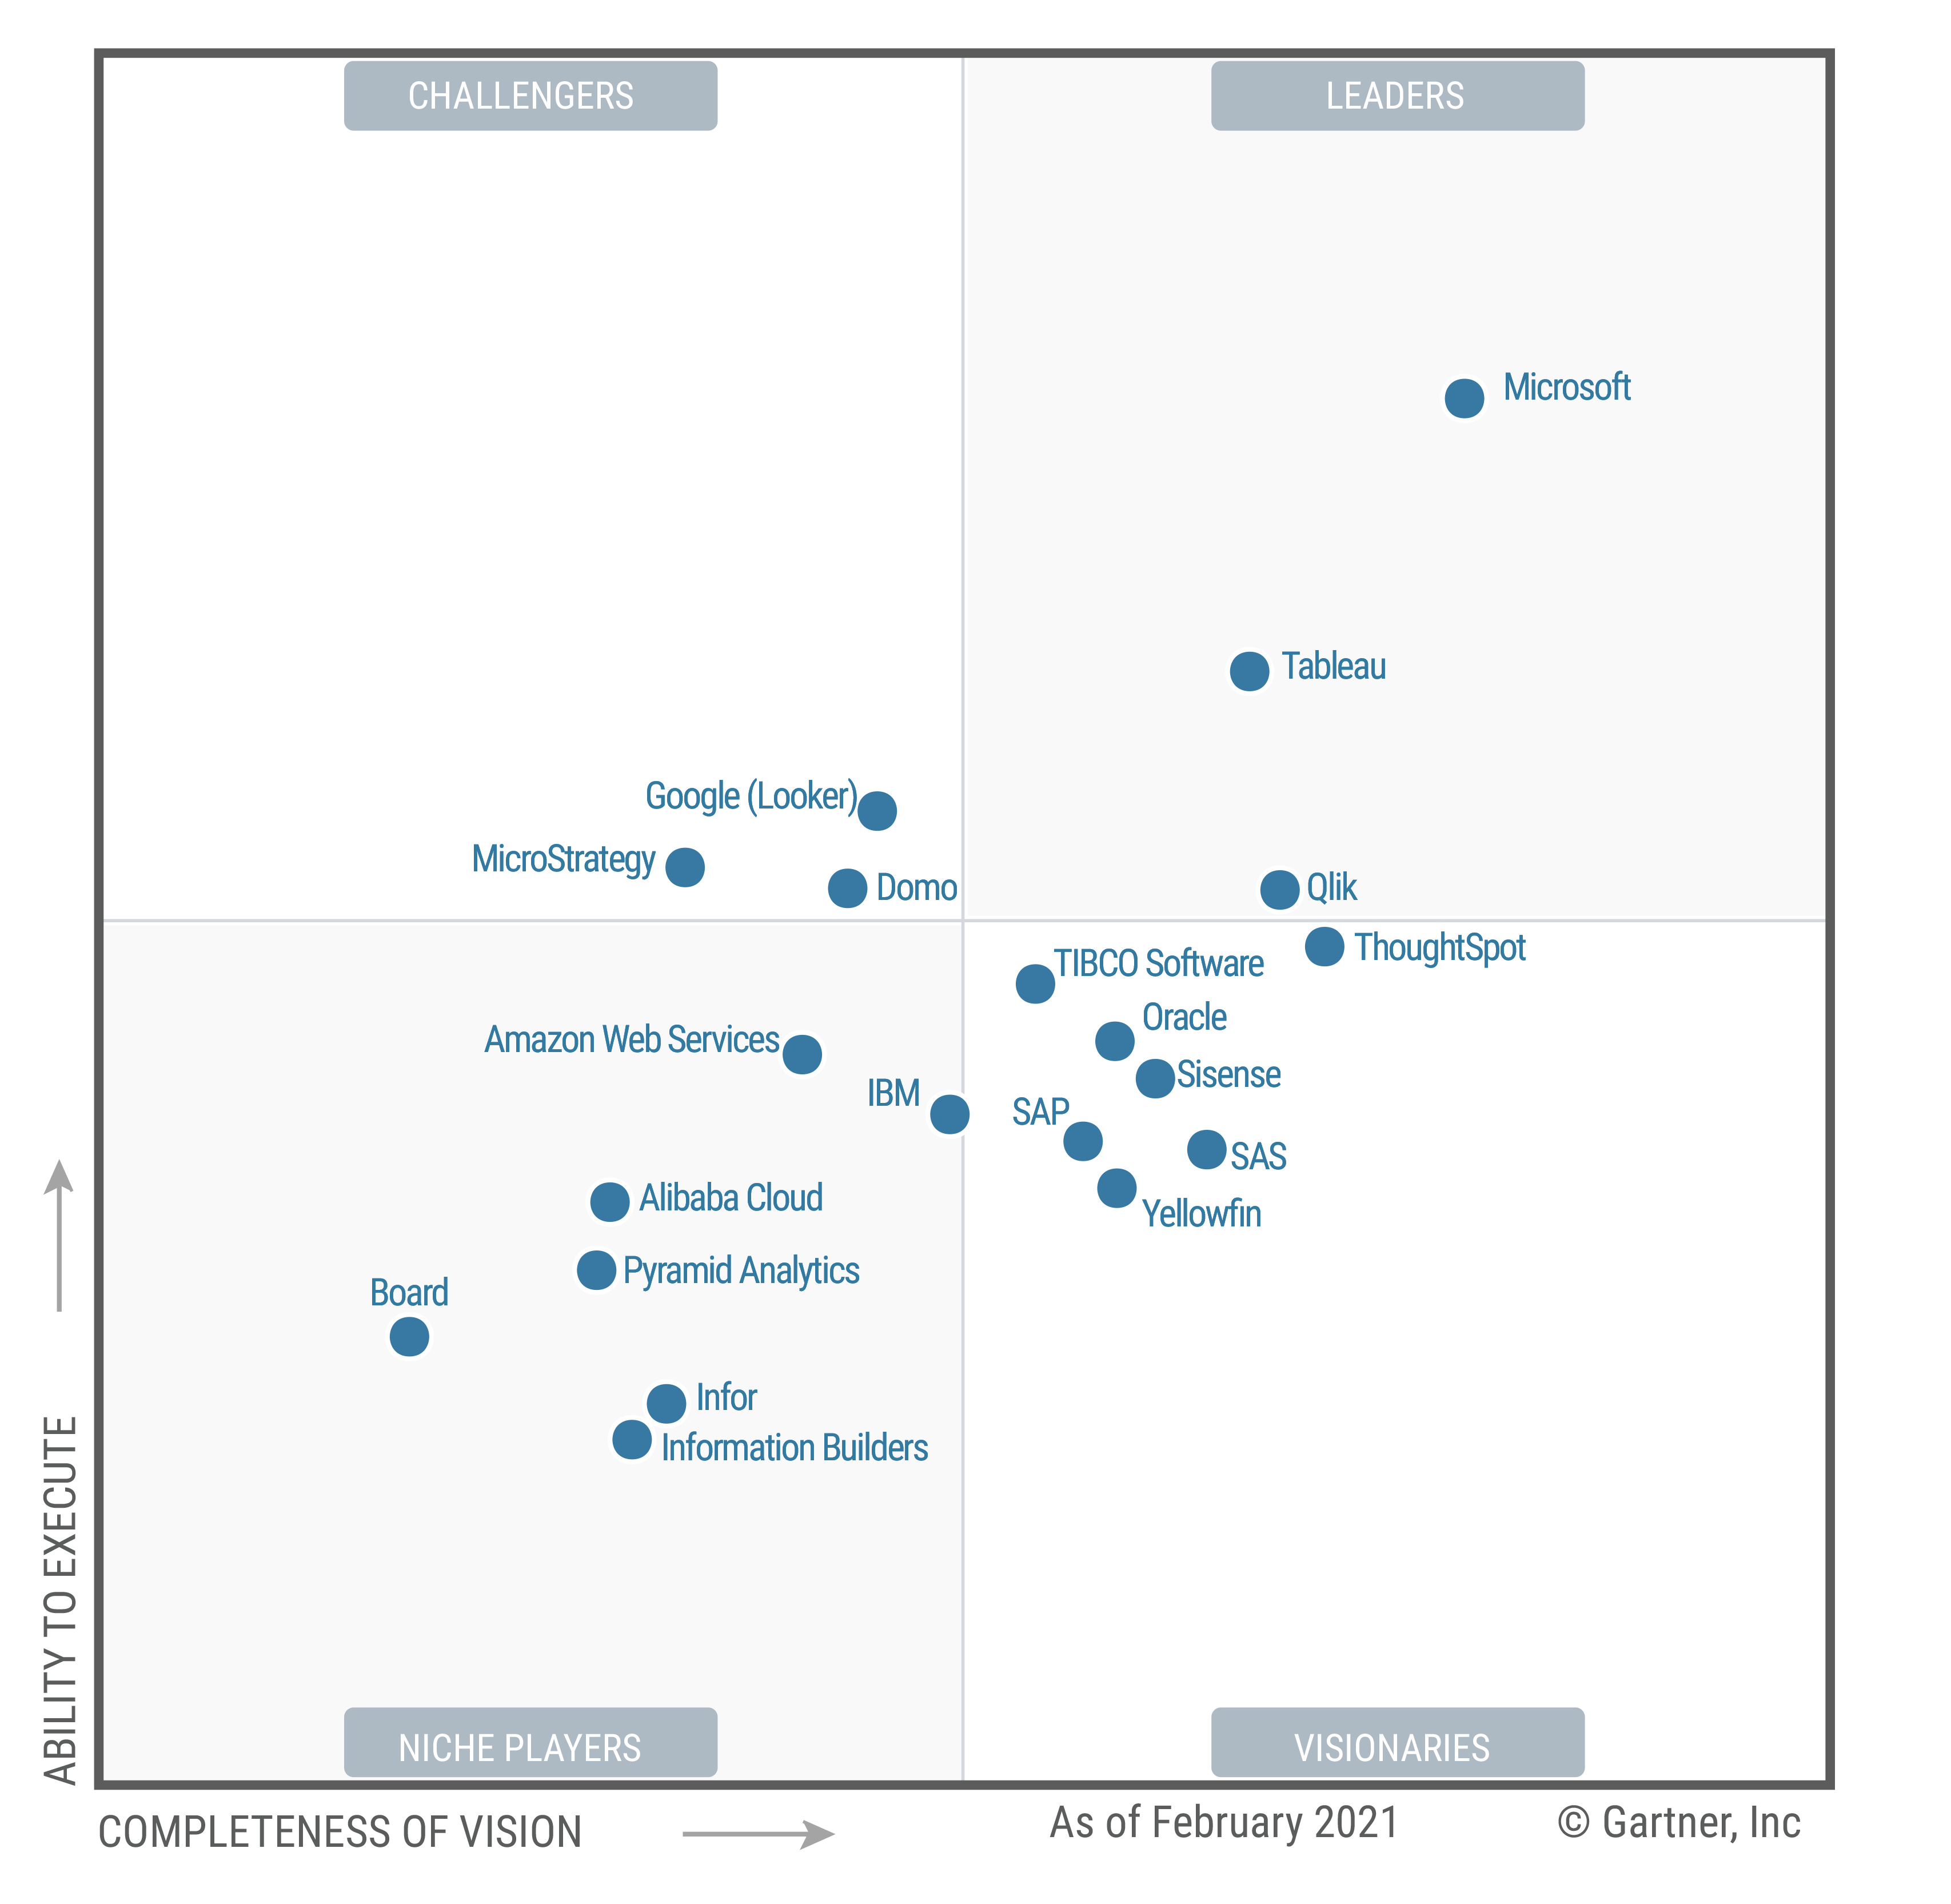
\includegraphics[width=0.6\linewidth]{img/gartner-BI-tools.png}
    \caption{Gartner BI Magic Quadrant, zdroj: Gartner, 2021}
    \label{fig:BITools}
\end{figure}

\textbf{TODO: Reference}



\subsection{Microsoft Power BI}

- představit templates 



\subsection{Tableau}
\subsection{Metabase}

SaaS deployment manažer
Vzpomenout ten v Go,
Mnoho nepotřebných features

\section{Závěr}\label{sec:AnalysEnd}

V předchozích sekcích jsme si představili několik nástrojů, jejichž kombinací lze splnit požadavky na funkcionalitu definované v~úvodním textu této kapitoly. 
Ovšem kombinace těchto nástrojů by vytvářela poměrně nesourodý celek, který by bylo složité automatizovat a~integrovat do jednoho systému.

Další problém představují nástroje na integraci dat.
Jsou totiž spíše určeny pro použití experty na integraci či analýzu dat, proto je u nich kladen důraz na obecnost a~širokou škálu využití, a~tak mnohonásobně převyšují požadovanou funkcionalitu pro náš systém.
Tato nepotřebná funkcionalita přidává na jejich komplexitě, což vytváří barieru pro použití ve spolupráci se zákazníkem - laikem.

V dalších kapitolách se tedy budeme soustředit na navržení a~implementaci vlastního řešení, které minimalizuje nabízenou funkcionalitu na nezbytně nutnou úroveň, jež splňuje funkční požadavky, za účelem zachování jednoduchosti použití.






%% Různých BI nástrojů, dále jen nástrojů, umožňujících vytváření reportů a~nástěnek existuje mnoho. 
%% Data jsou většinou importována přímo do těchto nástrojů nebo jsou nástroje napojeny na zákaznickou databázi.
%% Reporty si potom vytváří zákazník sám, či s~pomocí dodavatele software nebo specializovaných konzultantů. TODO: CITACE




